\documentclass{article}
\usepackage[utf8]{inputenc}
\usepackage[utf8]{inputenc}
\usepackage[english]{babel}
\usepackage{graphicx}
\usepackage{array}
\usepackage{underscore}
\usepackage{tabu}
\usepackage{float}
\usepackage{listings}
\usepackage{color}
\usepackage{tikz-uml}

\definecolor{dkgreen}{rgb}{0,0.6,0}
\definecolor{gray}{rgb}{0.5,0.5,0.5}
\definecolor{mauve}{rgb}{0.58,0,0.82}

\lstset{frame=tb,
  language=Python,
  aboveskip=3mm,
  belowskip=3mm,
  showstringspaces=false,
  columns=flexible,
  basicstyle={\small\ttfamily},
  numbers=none,
  numberstyle=\tiny\color{gray},
  keywordstyle=\color{blue},
  commentstyle=\color{dkgreen},
  stringstyle=\color{mauve},
  breaklines=true,
  breakatwhitespace=true,
  tabsize=3
}
\begin{document}
\begin{titlepage}
\begin{center}
\textsc{\LARGE Sharif University of Technology}\\[1.5cm]
\textsc{\Large A Simple Peer To Peer Network Implementation}\\[0.5cm]
\textsc{\large November 2018}\\
%----------------------------------------------------------------------------------------
%	AUTHOR SECTION
%----------------------------------------------------------------------------------------

\begin{minipage}{0.4\textwidth}
\begin{flushleft} \large
\emph{Authors:}\\
Hoora  \textsc{Abootalebi}\\
Nariman  \textsc{Aryan}\\
Amin \textsc{Isaai}\\
Amirhossein \textsc{Khajepour}\\
Mahdis \textsc{Tajdari}\\
Ali  \textsc{Zeynali} % Your name
\end{flushleft}
\end{minipage}
~
\begin{minipage}{0.4\textwidth}
\begin{flushright} \large
\emph{Supervisor:} \\
Dr. Mahdi \textsc{Jafari} % Supervisor's Name
\end{flushright}
\end{minipage}\\[2cm]
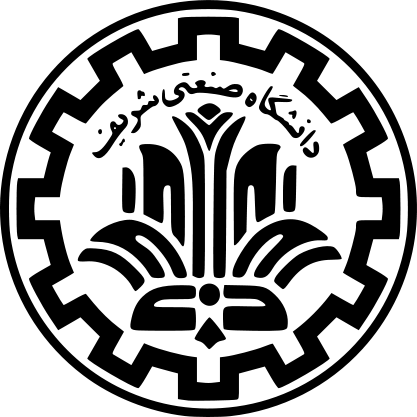
\includegraphics[scale=0.15]{sharif-logo.png}\\
\textbf{Computer Engineering Faculty}
\end{center}
\end{titlepage}
\large
\clearpage
\tableofcontents
\clearpage
\section{Introdeuction}
\paragraph{}This project aims to implement a peer to peer network. In the first step we design UML model and then we are going to explain each objects' attributes and methods. 
\section{UML model}
\paragraph{}We design the UML model in order to make the project more understandable, clearer and professional.
\\
\begin{tikzpicture}
%---------------------------Stream--------------------------
\umlclass[x=3, y=5, anchor=north]{Stream}{-_server_in_buf : dictionary \\+messages_dic :dict\\+nodes : dictionary\\+ip\\+port}{-__init__()\\+get\_server\_address()\\ +add\_node()\\+is\_valid()\\+remove\_node()\\+get\_node\_by\_server()\\+add\_message\_to\_out\_buff()\\+remove\_node\_by\_server\_info()\\+read\_in\_buf()\\+send\_messages\_to\_node()\\+send\_out\_buf\_messages()}

%--------------------------Packet Factory----------
\umlclass[x=-3, y=-2, anchor=north]{Packet Factory}{}{+parse\_buffer()\\+new\_reunion\_packet()\\+new\_advertise\_packet( )\\+new_join_packet()\\+new\_register\_packet()\\+new_message_packet()}

%----------------------------Peer--------------------------
\umlclass[x=0, y=-6, anchor=north]{Peer}{-\_is\_root\\+stream\\+parent\\+packets\\+neighbours\\-_user_interface\\-_user_interface_buffer\\-_broadcast_packets\\+packet_factory\\+network_nodes}{+start_user_interface()\\+handle_user_interface_buffer()\\+run()\\+handle_packet()\- __handle_advertise_packet()\\- __handle_register_packet()\\-  __handle_message_packet()\\-  __handle_reunion_packet()\\-__handle_join_packet()\\- __get_neighbour()}
%-----------------------------------------------------------
\umlassoc[arm2=-1.2cm]{Peer}{Packet Factory}
\umlassoc[arm2=-1.2cm]{Peer}{Stream}
\end{tikzpicture}
\clearpage
\begin{tikzpicture}
%------------------------------------------------------------------------
%----------------------------Packet-----------------------------------------
\umlclass[x=-4, y=-8, anchor=north]{Packet}{- _buf: \\- _header:\\-_version:\\-_type: String\\-_length: \\-_source_server_ip\\-_source_server_port\\-_body: String\\}{+ get\_header()\\+ get\_version()\\+ get\_type()\\+ get\_length()\\+ get\_body()\\+ get_buf()\\+ get_source_server_ip()\\+get_source_server_port()\\+get_source_server_address()}
%----------------------------Reunion----------------------------------------
%%\umlclass[x=+1.5, y=-11, anchor=north]{Reunion}{}{get\_destination()}
%----------------------------Advertise---------------------------------------
%%\umlclass[x=0, y=-14 ,anchor=north]{Advertise}{ip: String\\port: String}{}
%----------------------------Message----------------------------------------
%%\umlclass[x=-3, y=-14, anchor=north]{Message}{plain\_text : String}{}

%----------------------------Register Request------------------------------
%%\umlclass[x=-7, y=-14 ,anchor=north]{Register Request}{ip: String\\port: String}{}
%%\umlclass[x=+1.5, y=-11, anchor=north]{Reunion}{}{get\underline{\hspace{.05in}}destination()}  
%%\umlclass[x=0, y=-14 ,anchor=north]{Advertise}{ip: String\\port: String}{}  
%%\umlclass[x=-3, y=-14, anchor=north]{Message}{plain\underline{\hspace{.05in}}text : String}{}
%%\umlclass[x=-7, y=-14 ,anchor=north]{Register Request}{ip: String\\port: String}{}  
%%\umlclass[x=-9.5, y=-11, anchor=north]{Register Response}{ack : String}{}
%%\umlinherit[arm2=-1.2cm]{Reunion}{Packet} 
%%\umlinherit[arm2=-1.2cm]{Advertise}{Packet}
%%\umlinherit[arm2=-1.2cm]{Message}{Packet}
%%\umlinherit[arm2=-1.2cm]{Register Request}{Packet}
%%\umlinherit[arm2=-1.2cm]{Register Response}{Packet}
\end{tikzpicture}
\clearpage
\begin{tikzpicture}
%----------------------------User Interface---------------------------------
\umlclass[x=0, y=0, anchor=north]{userInterface}{}{}
%----------------------------Semi Node---------------------------------
\umlclass[x=3, y=0, anchor=north]{SemiNode}{}{-__inti__()\\+get_ip()\\+get_port()\\+get_address()\\+parse_ip()\\+parse_port()}
%----------------------------Graph Node---------------------------------
\umlclass[x=0, y=-2, anchor=north]{GraphNode}{}{-__init__()\\+set_parent()\\+set_address()\\-__reset()\\+add_child}
%----------------------------Network Node---------------------------------
\umlclass[x=3, y=-5, anchor=north]{NetworkGraph}{}{-__inti__()\\+find_live_node\\+find_node()\\+turn_on_node()\\+turn_off_node\\+remove_node()\\+add_node()}
%----------------------------Node--------------------------------------------
\umlclass[x=0, y=-10, anchor=north]{Node}{}{+ send_message()\\+add_message_to_out_buff()\\+close()\\+get_sever_address()\\+get_standard_server_address()\\+parse_ip()\\+parse_port()}
\end{tikzpicture}
\clearpage
\section{Objects}
\paragraph{}Now it's time to explain every obejct's duty.
\subsection{Stream}This objects has one server and n clients. Servers are always open for reading and clients will be open whenever we want to write on a socket. \\
There is a clientMsg dictionary in this object to handle messages. This means that there is an array assigned to a specific client for all clients. If we need to add a new client to this object, we use add\underline{\hspace{.05in}}client() method. Consequently, an array will be assigned to this new client in clientMsg.\\
There is also a remove\underline{\hspace{.05in}}client() method for the times when we want to remove a client from this object. This method is mostly used  when reunion fails.\\
The read\underline{\hspace{.05in}}inBuf returns the buffer of the server.\\
The send\underline{\hspace{.05in}}msg() method is used when peer wants to send a message to a specific client.\\
Byte\underline{\hspace{.05in}}ack() is used to reply to the receives messages. We must reply all of the receives messages by sending Ack (which is a string).\\
\begin{lstlisting}
#stream()

\end{lstlisting}
\paragraph{}We also need to add a dictionary to specify every client's message(s)
\subsection{Peer}This object is the main object that we are working with. It must have a Stream object which provides the connection to the socket; This means that reading and writing are done using the Stream object. Peer must also have a userInterface object in order to facilitate commanding by users.(.e.g. for connecting or sending message to a specific node)\\
The run method handles all of the events included in stream in an infinite loop and it also handles the received messages; This means that it does a certain action based on the type of the received packet.

\begin{lstlisting}
#Peer()
stream()
user_interface()   #Which the user or client sees and works with. 
run() 				#This method runs every time to see 
				     #whether there is new messages or not.
packetFactory()
handle_packets()
\end{lstlisting}
\subsection{Packet Factory}
\paragraph{packetFactory()}The main functionality of this object is to create different types of packet and return them. To be more specific, we read data from buffer and we pass it through pars\underline{\hspace{.05in}}buff() method in order to get a packet.
\begin{lstlisting}
#packetFactory
\end{lstlisting}
\subsection{Packet}

\paragraph{}Every packet consists seven differntes parts: \textbf{plain\_text} which is the raw text message in the packet.\\
\begin{lstlisting}
#Packet

\end{lstlisting}
\paragraph{}Every packet consists seven differntes parts: \textbf{plain\underline{\hspace{.05in}}text} which is the raw text message in the packet.\\
\textbf{Node}: Specifies to which node the packet sent to. \textbf{Sender} specifies who sent the packet \textbf{Validator} which makes the packet valid.\\ \textbf{Header} where the information such as type of the packet and etc. are going to be there.\\ \textbf{Body} body of our packet .
\subsection{Interface}
\paragraph{reunion(packet)} checks the connection of the nodes to the root. This is one type of packets which each node has to send it to the root every 20 seconds to clarify is still live. \\
A node who want to send reunion packet, after creating the header, inserts it's ip and port in the body and passes it to his father. Then the father should append it's ip and port at the end of the body then passes it to the next father... \\
When the root recieves the reunion packet from one node, the root should reverse the sort of ip and ports in the reunion's body then sets it as the reunion answer's body and pass it to the node which gave the reunion to the root. \\
Each node which receives the reunion answer from it's father, should check if the first ip and port in the body are for himself or not. If yes, it should pop his port and ip from the body and then send it to the next node which it's ip and port are in the top of the body.
This process continue until the destination node receives the reunion answer.
\begin{lstlisting}
#reunion(packet)
 get_destination()
\end{lstlisting}
\subsection{Node}
\begin{lstlisting}
#Node

\end{lstlisting}
\paragraph{}Every node has two parameters: \textbf{IP} and \textbf{Port}.
\subsection{Graph Node}
\paragraph{reg\underline{\hspace{.05in}}req()} sends IP/Port of a node to the root to ask if it can register it. 
\subsection{Network Node}
\paragraph{reg\underline{\hspace{.05in}}res()} should just send an from the root $Ack$ to inform a node that it has been registerd in the root if the reg\underline{\hspace{.05in}}req() was successful.
\subsection{Semi Node}
\paragraph{}
\subsection{}
\paragraph{}
\clearpage





\end{document}
